\documentclass[ignorenonframetext,xcolor=x11names]{beamer}

\definecolor{mun}{RGB}{134,38,51}
\definecolor{mun2}{RGB}{99,102,106}
%\definecolor{mun}{cmyk}{0,.3922,.2392,.1686}
\definecolor{code}{RGB}{0, 0, 128}
\definecolor{code}{gray}{0.95}

\mode<presentation>
{
%  \usetheme{boxes}
%  \usetheme{default}
%  \usetheme{Montpellier}
%  \usetheme{Singapore}
%   \usetheme{Rochester}
%  \usecolortheme{crane}
%  \usecolortheme{dolphin}
%  \usecolortheme{lily}
%  \usecolortheme{orchid}
  \usecolortheme{rose}
  \setbeamercovered{transparent}
%  \usefonttheme[onlymath]{serif}
  \setbeamercolor*{structure}{bg=mun,fg=mun}
  \setbeamercolor*{palette primary}{use=structure,fg=white,bg=structure.fg}
  \setbeamercolor*{palette secondary}{use=structure,fg=white,bg=structure.fg}
  \setbeamercolor*{palette tertiary}{use=structure,fg=white,bg=black}
  \setbeamercolor*{palette quaternary}{fg=white,bg=black}
  \setbeamercolor{section in toc}{fg=black,bg=white}
  \setbeamercolor{alerted text}{use=structure,fg=structure.fg!50!black!80!black}
  \setbeamercolor{titlelike}{parent=palette primary,fg=structure.fg!50!black}
  \setbeamercolor{frametitle}{bg=mun,fg=white}
  \setbeamercolor*{titlelike}{parent=palette primary}

  \setbeamercolor{normal text}{fg=black!90}
  \setbeamercolor{math text}{fg=black}
  \setbeamercolor{quote}{bg=gray!20}
  \setbeamercolor{quotation}{bg=gray!20}
  \setbeamerfont{cite}{size=\scriptsize}
  \setbeamerfont{quote}{size=\footnotesize}
  \setbeamerfont{quotation}{size=\footnotesize}
  \setbeamercolor{red text}{fg=red!75!black}
  \setbeamertemplate{bibliography item}[triangle]
  \setbeamertemplate{enumerate item}[square]
  \setbeamertemplate{blocks}[rounded][shadow=true]
  \setbeamertemplate{navigation symbols}{}
  \setbeamertemplate{footline}[frame number]
}
\usepackage{tcolorbox}
\usepackage{amsmath}
\usepackage{physics}
\usepackage{pgf}
\usepackage[english]{babel}
\usepackage[latin1]{inputenc}
\usepackage{times}
\usepackage[T1]{fontenc}
\usepackage{multicol}
\usepackage{multirow}
\usepackage{fancyvrb}
\usepackage{tabularx}
\usepackage{amsmath}
\usepackage{bbm}
\usepackage{alltt}
\usepackage{hyperref}
\hypersetup{
    colorlinks=true,
    linkcolor=blue,
    filecolor=magenta,      
    urlcolor=blue,
}
\usepackage{minted}
\newminted{cypher}{autogobble,bgcolor=code,breakbytoken,frame=single,framesep=3pt}
\newminted{R}{autogobble,bgcolor=code,breakbytoken,frame=single,framesep=3pt}
\newminted{text}{autogobble,bgcolor=code,breakbytoken,frame=single,framesep=3pt}
\newminted{sql}{autogobble,bgcolor=code,breakbytoken,frame=single,framesep=3pt}
\newminted{bash}{autogobble,bgcolor=code,breakbytoken,python3,frame=single,framesep=3pt}
\newminted{xml}{autogobble,bgcolor=code,breakbytoken,python3,frame=single,framesep=3pt}
\newminted{python}{bgcolor=code,breakbytoken,python3,frame=single,framesep=3pt}
\newminted{html}{autogobble,bgcolor=code,breakbytoken,frame=single,framesep=3pt}
\newminted{js}{autogobble,bgcolor=code,breakbytoken,frame=single,framesep=3pt}
\AtBeginEnvironment{minted}{%
  \renewcommand{\fcolorbox}[4][]{#4} \scriptsize}
\AtEndEnvironment{minted}{%
  \normalsize}

%\newcommand{\Pr}{\operatorname{Pr}}
\newcommand{\argmax}{\operatorname*{argmax}}
\newcommand{\argmin}{\operatorname*{argmin}}
\newcommand{\Ident}{\operatorname{I}}

\author % (optional, use only with lots of authors)
{Joerg Evermann}
% - Give the names in the same order as the appear in the paper.
% - Use the \inst{?} command only if the authors have different
%   affiliation.

\institute%[Universities of Somewhere and Elsewhere] % (optional, but mostly needed)
{
  Faculty of Business Administration\\
  Memorial University of Newfoundland \\ 
  \texttt{jevermann@mun.ca} 
}

\date{}

\pgfdeclareimage[width=1.5cm]{university-logo}{../MUN_LOGO_CMYK}
\logo{\pgfuseimage{university-logo}}

% If you wish to uncover everything in a step-wise fashion, uncomment
% the following command: 

%\beamerdefaultoverlayspecification{<+->}

 
\title{Business 4720 - Class 5}

\subtitle{Data Management in R using Tidyverse}

\begin{document}

\begin{frame}{}
  \titlepage
  \footnotesize
  \begin{center}

\includegraphics[height=.5in]{../by-nc.png}

Unless otherwise indicated, the copyright in this material is owned by Joerg Evermann. This material is licensed to you under the \href{https://creativecommons.org/licenses/by-nc/4.0/}{Creative Commons by-attribution non-commercial license (CC BY-NC 4.0)}
\end{center}

\end{frame}

\section{Introduction}

\begin{frame}{This Class}

\begin{block}{What You Will Learn:}
\begin{itemize}
  \item Introduction to R
  \item Introduction to the Tidyverse set of packages
  \begin{itemize}
  \item ''Tidy'' data
  \item Manipulating \& clearning data
  \item Joining data
  \item Summarizing and reporting data
  \end{itemize}
  \item Data cleaning
\end{itemize}
\end{block}
\end{frame}

\section{R}

\begin{frame}{Intro to R}
\begin{block}{What is R?}
\begin{itemize}
  \item System for statistical analyses
  \item Created in 1993
  \item R programming language
  \item Open-source, cross-platform
  \item Widely used, popular
  \item Extensible, thousands of packages
  \item Scripting and programming
\end{itemize}  
\end{block}
\vspace{5mm}
\textbf{Intro Tutorial:}
\url{https://cran.r-project.org/doc/manuals/r-release/R-intro.pdf}
\end{frame}

\begin{frame}{R}
\centering
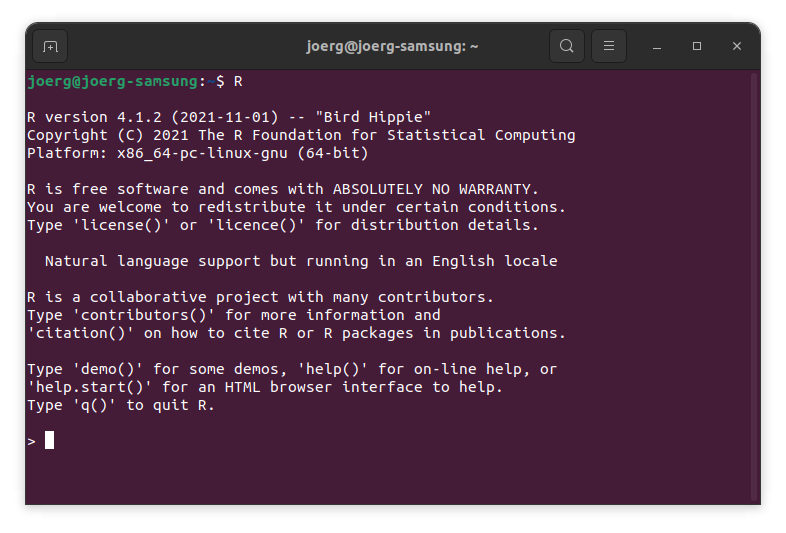
\includegraphics[width=\textwidth]{screen1.png}
\end{frame}

\begin{frame}[fragile]{My First R Command}
R can do math:
\begin{Rcode}
> 1+1
[1] 2
\end{Rcode}
R knows variables:
\begin{Rcode}
> a <- 3
> b <- 2
> print(a * b)
[1] 6
\end{Rcode}
\emph{Note}: You can also assign using ''=''
\end{frame}

\begin{frame}[fragile]{R Basics}
R does vector math:
\begin{Rcode}
> v <- c(1, 2, 3, 4)
> v*3
[1]  3  6  9 12
\end{Rcode}
\emph{Note}: No print statement needed in interactive mode\\

\begin{Rcode}
> s <- seq(0, 6, by=.5)
> print(s)
> r <- rep(3.5, 5)
> print(r)
\end{Rcode}
\end{frame}

\begin{frame}[fragile]{R Basics \small [cont'd]}
More basic functions on vectors:
\begin{Rcode}
> length(v)
> max(v)
> min(v)
> sqrt(vv)
> var(v)
> sd(v)
> vv <- c(v, c(7, 8, 9), v)
> print(vv)
\end{Rcode}
\end{frame}

\begin{frame}[fragile]{R Basics \small [cont'd]}
Vector indexing:
\begin{Rcode}
> vv[vv < 5]
> vv[vv < 5] <- vv[vv < 5] + 5
> vv[3:7]
> vv[-(3:7)]
\end{Rcode}
\end{frame}

\begin{frame}[fragile]{R Basics \small [cont'd]}
R knows if its not a number:
\begin{Rcode}
> 2 / 0
[1] Inf
> 0 / 0
[1] NaN
\end{Rcode}
\end{frame}

\begin{frame}[fragile]{R Basics \small [cont'd]}
R knows NA:
\begin{Rcode}
> v[3] <- NA
> v*3
[1]  3  6 NA 12
> is.na(v)
[1] FALSE FALSE  TRUE FALSE
> sum(v)
[1] NA
\end{Rcode}
\emph{Note}: R indexes start at 1! \\
\emph{Note}: TRUE and FALSE can be abbreviated T and F \\
\end{frame}

\begin{frame}[fragile]{R Basics \small [cont'd]}
R knows boolean logic:
\begin{Rcode}
> TRUE & FALSE
FALSE
> TRUE | FALSE
TRUE
\end{Rcode}
R know character strings:
\begin{Rcode}
> label1 = 'I Love R'
> label2 = 'and BUSI 4760'
> paste(label1, label2, sep=' ')
> strsplit('Hello World! My first string', ' ')
\end{Rcode}
\end{frame}

\begin{frame}[fragile]{R Basics \small [cont'd]}
R types and type coercion:
\begin{Rcode}
> is.numeric(vv)
> is.integer(vv)
> mode(vv)
> as.character(vv)
> is.character(as.character(vv))
> as.factor(as.character(vv))
> levels(as.factor(as.character(vv)))
\end{Rcode}
\end{frame}

\begin{frame}[fragile]{R Environment}
R can manipulate its objects (''workspace'')
\begin{Rcode}
> ls()
[1] "a"          "b"          "v"
> rm(v)
> ls()
[1] "a"          "b"
\end{Rcode}
\end{frame}

\begin{frame}[fragile]{R Basics \small [cont'd]}
R knows Regex:
\footnotesize
\begin{Rcode}
> grep('^([0-9]{3})[ -]?[0-9]{3}[ -]?[0-9]{4}$', 
    c('709 864 5000', 'abc def 9999', '709-865-5000'))
[1] 1 3
> grep('[A-V][0-9][A-V] [0-9][A-V][0-9]', 
    c('A0P 1L0', '0AB L2K', 'A0X 1Z0'))
[1] 1
\end{Rcode}
\normalsize
R knows Levenshtein distances:
\footnotesize
\begin{Rcode}
> agrep('apple', 
    c('apricot', 'banana', 'grape', 'pineapple'), 
    max.distance=3)
[1] 1 3 4
\end{Rcode}
\end{frame}

\section{The R Environment}

\begin{frame}[fragile]{R Environment \small [cont'd]}
R can help:
\begin{Rcode}
> help()
> help(lm)
> ?lm
> ??lm
> help.start()
\end{Rcode}
\end{frame}

\begin{frame}[fragile]{R Environment \small [cont'd]}
R knows files and directories:
\begin{Rcode}
> getwd()
[1] "/home/busi4720"
> setwd('DataSets')
> getwd()
[1] "/home/busi4720/DataSets"
> list.files()
\end{Rcode}
\emph{Note}: Strings may be enclosed in double or single quotes. \\
\end{frame}

\begin{frame}[fragile]{R Environment \small [cont'd]}
R uses packages:
\begin{Rcode}
> search()
> library(matrixcalc)
> search()
> library()
> install.packages('lavaan')
> library()
> installed.packages()
\end{Rcode}
R can read your command files:
\begin{Rcode}
> source('MyFirstScript.R')
\end{Rcode}
\emph{Note}: Sourcing a script turns off auto-printing, you must use explicit \texttt{print()} commands
\end{frame}

\begin{frame}[fragile]{R Environment \small [cont'd]}
Say goodbye to R:
\begin{Rcode}
> quit()
\end{Rcode}
R stores its \textbf{workspace} in each directory in a file called ''.RData'' and will read it when restarted. R stores its \textbf{command history} in each directory in a file called ''.Rhsitory'' and will read it when restarted.
\end{frame}

\begin{frame}[fragile]{R Arrays and Matrices}
Arrays and matrices have dimensions:
\begin{Rcode}
> a <- array(1:20, dim=c(4,5))
> a
     [,1] [,2] [,3] [,4] [,5]
[1,]    1    5    9   13   17
[2,]    2    6   10   14   18
[3,]    3    7   11   15   19
[4,]    4    8   12   16   20
> a[,2]
> a[,2:4]
> a[3,2:4]
> a[3:1,2:4]
> i <- array(c(1:3,3:1), dim=c(3,2))
> a[i] <- 0
> a
\end{Rcode}
\end{frame}

\begin{frame}[fragile]{R Arrays and Matrices \small [cont'd]}
\begin{Rcode}
> b <- matrix(20:1, nrow=5, byrow=T)
> b
     [,1] [,2] [,3] [,4]
[1,]   20   19   18   17
[2,]   16   15   14   13
[3,]   12   11   10    9
[4,]    8    7    6    5
[5,]    4    3    2    1
> is.matrix(b)
> is.matrix(a)
> t(b)
> cbind(a, t(b))
> rbind(t(a), b)
\end{Rcode}
\end{frame}


\begin{frame}[fragile]{R Lists}
R knows lists:
\begin{Rcode}
> l <- list('a', 3, 'b', 2, TRUE)
> l[[2]]
> l[2]
> is.list(l)
> is.list(l[[2]])
> is.list(l[2])
> as.list(vv)
\end{Rcode}
\emph{Vectors are not lists}: Lists can contain elements of different types, vectors cannot:
\begin{Rcode}
> c(3, 'a', TRUE)
> c(3, FALSE, TRUE)
\end{Rcode}
\end{frame}


\begin{frame}[fragile]{Data Frames}
A dataframe is a special type of list:
\begin{Rcode}
> x <- rnorm(50)
> y <- 2*x + rnorm(50)
> data <- data.frame(x, y)
> colnames(data)
> colnames(data) <- c('Pred', 'Crit')
> nrow(data)
> ncol(data)
> data$Pred
> data$Crit
> summary(data)
> head(data)
> tail(data)
> cov(data)
\end{Rcode}
\end{frame}


\begin{frame}[fragile]{Data Frames \small [cont'd]}
Writing data to CSV:
\begin{Rcode}
> write.csv(data, 'data.csv', row.names=FALSE)
\end{Rcode}

Reading data from CSV:
\begin{Rcode}
> new.data <- read.csv('data.csv')
> colnames(new.data)
\end{Rcode}
\end{frame}

\begin{frame}{Tips for Working with R}
\begin{itemize}
    \item Use the \colorbox{lightgray}{up-arrow} key to retrieve earlier commands
    \item The \texttt{history()} function shows your command history
    \item Use a notepad app to assemble your commands, then copy/paste to R
    \item Use a notepad app for your results, copy/paste from R
    \item The Ubuntu terminal window uses \colorbox{lightgray}{SHIFT-CTRL-X}, \colorbox{lightgray}{SHIFT-CTRL-C}, \colorbox{lightgray}{SHIFT-CTRL-V}
    \item Use multiple R windows (e.g. one for executing commands, one for reading help documentation or listing files)
    \item Don't update packages in the middle of a project
    \item Ensure you have a \emph{repeatable, automatable script} for your entire data analysis at the end of a project
\end{itemize}
\end{frame}

\begin{frame}{Hands-On Exercise}
\begin{enumerate}
   \item Consider the last five digits of your student ID and label those digits A--E
   \begin{itemize}
      \item Example: Student ID=12453 $\Rightarrow$ A=1, B=2, C=4, D=5, E=3
   \end{itemize}
   \item Create a data frame with $(A+1)$ columns and $10*(B+1)$ rows of random numbers with mean of $C$ and standard deviation of $(D+1)$ (use the \texttt{rnorm()} function)
   \item Name the columns with letters from ''A''--''K''
   \item ''Clip'' the values so that all values lie between $-(E+1)$ and $+(E+1)$
   \item Summarize the data and print the pairwise covariance matrix of the variables in the data frame
   \item Save the data frame in a CSV file using your first name as file name (file ending '.csv')
   \item Save your script in an R file using your first name as file name (file ending '.R')
\end{enumerate}
\end{frame}

\section{Tidyverse}

\begin{frame}{Tidyverse}
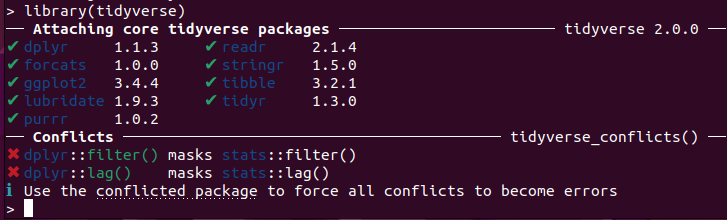
\includegraphics[width=\textwidth]{screen2.png}\\

\textbf{Intro books}: \url{https://r4ds.hadley.nz/}
\end{frame}

\begin{frame}{Tidyverse}
\renewcommand{\arraystretch}{1.25}
\centering

\begin{tabular}{l|l} \hline
dplyr & Manipulate data \\
forcats & Work with categorical variables (factors) \\
ggplot2 & Grammar of Graphics \\
lubridate & Date and time parsing and arithmetic \\
purrr & Functional programming \\
readr & Read files in various formats \\
stringr & Work with character strings \\
tibble & A tibble is better than a table \\
tidyr & Make data tidy \\ \hline
\end{tabular}
\end{frame}

\begin{frame}[fragile]{Pagila Database in R}
Read into a tibble:
\small
\begin{Rcode}
rentals <- read_csv('rentals.csv')
head(rentals)
summary(rentals)
\end{Rcode}
Fix the column datatypes:
\footnotesize
\begin{Rcode}
attach(rentals)
rating <- as.factor(rating)
language <- as.factor(language)
customer_address <- as.integer(customer_address)
customer_store <- as.integer(customer_store)
rental_staff <- as.integer(rental_staff)
payment_staff <- as.integer(payment_staff)
rental_duration <- as.integer(rental_duration)
detach(rentals)
summary(rentals)
\end{Rcode}
\end{frame}

\begin{frame}[fragile]{Pagila Database in R \small [cont'd]}
Examine the NA's:
\footnotesize
\begin{Rcode}
rentals |> 
  filter(if_any(everything(), is.na)) |>
  select(last_name, rental_date, return_date, 
         title, amount) |>
  print(n=Inf, width=Inf)
\end{Rcode}
\normalsize
\emph{Interpretation:}
\begin{itemize}
  \item Some films have not been rented
  \item Some rentals have not been returned
\end{itemize}
\emph{Notes:}
\begin{itemize}
  \item The pipe symbol (R native pipes \texttt{|>} or magrittr pipes \texttt{\%>\%})
  \item No quoting of column names
\end{itemize}
\end{frame}

\begin{frame}[fragile]{Pagila Database in R \small [cont'd]}

Find all films and the actors that appeared in them, ordered by film category and year, for those films that are rated PG:

\scriptsize
\begin{Rcode}
actors <- read_csv('actors.categories.csv')

rentals |> 
    full_join(actors, 
        by='title', 
        suffix=c('_customer', '_actor'), 
        relationship='many-to-many') |>
    filter(rating == 'PG') |>
    mutate(actor = 
        paste(last_name_actor, ', ', 
        first_name_actor, sep='')) |>
    rename(year=release_year) |>
    select(actor, title, category, year) |>
    distinct(actor, title, category, year) |>
    group_by(category, year, title) |> 
    nest() |>
    arrange(category, year, title) |>
    relocate(category, year, title) |>
    print(n=Inf, width=Inf)
\end{Rcode}
\end{frame}

\begin{frame}{Summary of DPlyr ''Verbs'' so far}
\centering
\renewcommand{\arraystretch}{1.25}

\begin{tabular}{l|l} \hline
full\_join & outer join (also left\_join, inner\_join, right\_join) \\
filter & filters by row \\
select & selects columns to retain \\
mutate & creates new columns \\
rename & renames columns \\
distinct & finds unique values \\
group\_by & groups data \\
nest & nests data, tibbles in tibbles \\
arrange & sorts data rows \\
relocate & moves data columns \\
print & prints a tibble \\ \hline
\end{tabular}
\end{frame}

\begin{frame}[fragile]{Pagila Database in R \small [cont'd]}

Find the most popular actors in the rentals in each city:

\scriptsize
\begin{Rcode}
addresses <- read_csv('addresses.csv')
addresses$phone <- as.character(addresses$phone)

rentals |> 
   inner_join(addresses,
       by=c('customer_address'='address_id')) |>
   inner_join(actors,
       by='title',
       suffix=c('_customer', '_actor'),
       relationship='many-to-many') |>
   mutate(actor = 
       paste(last_name_actor, ', ', 
       first_name_actor, sep='')) |>
   group_by(city, actor) |>
   summarize(count=n()) |>
   mutate(ranking = min_rank(desc(count))) |>
   filter(ranking < 4) |>
   arrange(city, ranking, actor) |>
   print(n=25)
\end{Rcode}

\normalsize
\emph{Note}: Use \texttt{rank()} to break ties, \texttt{dense\_rank()} for no gaps
\end{frame}

\begin{frame}[fragile]{Pagila Database in R \small [cont'd]}

Find the customers who spend the most on rentals, with their phone numbers and cities, and the number of rentals with the higest total rental payments for each category grouped by rental duration.

\footnotesize
\begin{Rcode}
full_data <- 
   rentals |> 
     inner_join(addresses,
       by=c('customer_address'='address_id')) |>
     inner_join(actors,
       by='title',
       suffix=c('_customer', '_actor'),
       relationship='many-to-many')
\end{Rcode}
\end{frame}

\begin{frame}[fragile]{Pagila Database in R \small [cont'd]}
\footnotesize
\begin{Rcode}
full_data |>
   mutate(customer=
     paste(first_name_customer, last_name_customer)) |>
   select(customer, amount, rental_duration, 
          category, phone, city) |>
   group_by(category, rental_duration, customer ) |>
   mutate(payments=sum(amount), num_rentals=n()) |>
   select(-amount) |>
   group_by(category, rental_duration) |>
   mutate(ranking = min_rank(desc(payments))) |>
   slice(which.min(ranking)) |>
   print(n=Inf, width=Inf)
\end{Rcode}
\normalsize

\begin{itemize}
  \item No \texttt{summarize()}
  \item ''Negative'' \texttt{select()}
  \item Multiple \texttt{group\_by()}
  \item Uses \texttt{slice()}
\end{itemize}
\end{frame}

\begin{frame}[fragile]{Pagila Database in R \small [cont'd]}
Get the total rental revenue, number of rentals, and the mean and standard deviation of the rental amounts for each country.

\footnotesize
\begin{Rcode}
full_data |>
  group_by(country) |>
  summarize(revenue=sum(amount), 
            numrentals=n(),
            mean_amount=mean(amount),
            sd_amount=sd(amount)) |>
  arrange(desc(mean_amount),
          desc(revenue)) |>
  print(n=Inf, width=Inf)  
\end{Rcode}
\normalsize
\end{frame}

\begin{frame}[fragile]{Pagila Database in R \small [cont'd]}
Get the top 5 and the bottom 5 grossing customers for each quarter.

\footnotesize
\begin{Rcode}
full_data |>
  mutate(customer=
   paste(first_name_customer,last_name_customer)) |>
  mutate(q=
   as.character(quarter(rental_date, with_year=T))) |>
  select(customer, q, amount, rental_date) |>
  group_by(q, customer) |>
  mutate(payments=sum(amount)) |>
  select(-amount) |>
  distinct(customer, q, payments) |>
  group_by(q) |>
  mutate(rank_top = min_rank(desc(payments))) |>
  mutate(rank_bot = min_rank(payments)) |>
  filter(rank_top < 6 | rank_bot < 6) |>
\end{Rcode}
\end{frame}

\begin{frame}[fragile]{Pagila Database in R \small [cont'd]}
Continued from previous slide \ldots

\footnotesize
\begin{Rcode}
  arrange(q, desc(payments)) |>
  relocate(q, customer, payments, 
              rank_top, rank_bot) |>
  print(n=Inf, width=Inf)
\end{Rcode}
\normalsize
\begin{itemize}
  \item No \texttt{summarize()}
  \item Uses \texttt{quarter()} function from package \texttt{lubridate}
  \item Uses \texttt{filter()} instead of slice \texttt{slice()}
\end{itemize}
\end{frame}


\begin{frame}[fragile]{Pagila Database in R \small [cont'd]}

Find the set of film titles by rental customer and the total number rentals for each customer

\footnotesize
\begin{Rcode}
full_data |>
  mutate(customer=
    paste(first_name_customer,last_name_customer)) |>
  select(customer, title) |>
  nest(titles=title) |>
  rowwise() |> 
  mutate(rentals=nrow(titles)) |>
  mutate(unique_titles=list(distinct(titles))) |>
  select(-titles) |>
  arrange(customer)
\end{Rcode}
\normalsize

\begin{itemize}
  \item Work with nested data using \texttt{nest} and \texttt{rowwise}
\end{itemize}
\end{frame}


\begin{frame}{Hands-On Exercises}
\begin{enumerate}
  \item Find all films with a rating of 'PG'
  \item List all customers who live in Canada (with their address)
  \item Find the average \emph{actual} rental duration for all films
  \begin{itemize}
     \item This requires date arithmetic, use the \texttt{lubridate} package
  \end{itemize}
  \item Find the average overdue time for each customer
  \begin{itemize}
     \item This requires date arithmetic, use the \texttt{lubridate} package
  \end{itemize}
  \item List all films that have never been rented
  \item List the names of actors who have played in more than 15 films
\end{enumerate}
\end{frame}

\begin{frame}[fragile]{R knows SQL}

\begin{block}{The \texttt{sqldf} Package}
  \begin{itemize}
     \item Set up an in-memory SQLite database (or use existing database connection)
     \item Move dataframes to database tables
     \item Run SQL query against database
     \item Move result set to R dataframe
     \item Tear down the in-memory database (optional)
  \end{itemize}
\end{block}

\begin{block}{Example}
\small
\begin{Rcode}
library(sqldf)
result_df <- 
   sqldf('select distinct(title) from full_data')
\end{Rcode}
\end{block}
\end{frame}


\begin{frame}{SQL Databases versus R/Tidyverse}
\begin{block}{Consider:}
  \begin{itemize}
     \item \textbf{Size of data}: R is memory limited, RDBMS scale massively larger
     \item \textbf{Access speed}: RDBMS have sophisticated indexes and query planners
     \item \textbf{Currency}: Operational system RDBMS has live data
     \item \textbf{Transactions}: RDBMS ensure consistent views of data across multi-user, concurrent updates
     \item \textbf{Impact}: Queries impact transaction processing (updates of data) performance in RDBMS 
     \item \textbf{Tools}: R has tools for statistical analysis and visualization, beyond mere reporting
  \end{itemize}
\end{block}
\end{frame}

\begin{frame}{SQL Databases versus R/Tidyverse \small [cont'd]}
\begin{block}{Recommendations:}
  \begin{itemize}
     \item Do not ''hit'' operational RDBMS for heavy-weight or frequent analytics
     \item Regularly export consistent data from RDBMS
     \item Use separate in-memory or on-disk RDBMS for analytics (e.g. with \texttt{sqldf}) if desired/required
     \item If size of data is large, consider distributed tools such as Hadoop/Spark
  \end{itemize}
\end{block}
\end{frame}



\begin{frame}{Data Cleaning}

\begin{block}{Overview}
\begin{itemize}
  \item Critical step in the data analysis process
  \item Identification and rectification of errors and inconsistencies
  \item Improve data quality
\end{itemize}
\end{block}
\end{frame}

\begin{frame}{Data Cleaning}
\begin{itemize}
  \item Critical step in the data analysis process
  \item Identify and ''fix'' errors and inconsistencies
  \item Improve data quality
\end{itemize}

\begin{block}{Activities}
\begin{enumerate}
    \item \textbf{Auditing}: Identify anomalies and inconsistencies

    \item \textbf{Validation}: Ensure data conforms to rules and constraints

    \item \textbf{Cleaning:} Transform and correct data

    \item \textbf{Duplicate Removal:} Ensure uniqueness of data.

    \item \textbf{Harmonization:} Merge datasets from different sources and ensure consistent formats and scales.

    \item \textbf{Standardization:} Bring data into a standard format.

    \item \textbf{Quality Assessment:} Ensure cleaning has been effective.
\end{enumerate}
\end{block}
\end{frame}

\begin{frame}{Data Validation}
\begin{itemize}
 \item Coding/serialization rules, e.g. with Regex 
 \begin{itemize}
   \item \textbf{Example} Are all phone numbers of the format: 
   \colorbox{code}{\texttt{\footnotesize \Verb_^([0-9]{3})[ -]?[0-9]{3}[ -]?[0-9]{4}$_}}
 \end{itemize}
 \item Data type constraints
 \begin{itemize}
   \item \emph{Example}: Are all sales prices numbers?
 \end{itemize}
 \item Range constraints
 \begin{itemize}
   \item \emph{Examples}: Are prices $> 0$? Are sales number $< 1000$?
 \end{itemize}
 \item Cross-field validation
 \begin{itemize}
   \item \emph{Example}: If province is NL, then area code must be 709
 \end{itemize}
 \item Uniformity of measures/scales
 \begin{itemize}
   \item \emph{Example}: All weights must be in kg, not pounds
 \end{itemize}
\end{itemize}
\end{frame}

\begin{frame}{Data Validation \small [cont'd]}
\begin{itemize}
 \item Uniqueness constraints
 \begin{itemize}
   \item Real duplicates and synonyms
   \item \emph{Example}: Rebekah Uqi Williams \\ (Commissioner of Nunavut (2020--2021)
   \item \textbf{Abbreviations}: \\ Rebekah U. Williams; Rebekah Williams, R.U. Williams
   \item \textbf{Order}: \\ Williams, Rebekah Uqi; Williams, Rebekah U.; Williams, R.
   \item \textbf{Spelling}: \\ Rebekah; Rebecca; Rebeccah; Rebeckah; Rebecka
   \item \textbf{Misspellings}: \\ Reebkah, Rebkah, Wililams, Willaims, \ldots
   \item \ldots
 \end{itemize}
\end{itemize}
\end{frame}

\begin{frame}{Data cleaning}
\begin{itemize}
	\item \textbf{Data Transformation,} into proper format or structure.
	\begin{itemize}
	  \item One row for each observation, case, event, \ldots
	  \item Requires case or event identifiers
	\end{itemize}
	\item \textbf{Data Imputation,} replacing missing values with estimated or default values, or removing missing values
	\begin{itemize}
	  \item Different meanings of missing values
	  \item Removal may bias data
	  \item Estimating values may be error-prone
	\end{itemize}
	\item \textbf{Data Correction,} or removal of erroneous data.
	\begin{itemize}
	  \item Requires access to correct data
	\end{itemize}
\end{itemize}
\end{frame}

\begin{frame}{Data Cleaning}
\begin{block}{Important}
Cleaning, transformation, and correction of data is \emph{subjective} and requires \emph{expert knowledge} of the data, the validation rules, the metadata, and the application domain.
\end{block}
\vspace{5mm}
\begin{block}{The 80/20 Rule of Data Science}
Cleaning, transformation, and correction of data takes 80\% of of the time, data analysis takes 20\% of the time.
\end{block}
\end{frame}

\end{document}
